% !TEX root = Apostila GP.tex

\chapter{Ferramentas de TI}

\section{Microsoft Project}

Um dos \sws mais conhecidos de gerenciamento de projetos, se destaca pela sua facilidade de utilização. Aqui apresentaremos algumas das principais funcionalidades da versão 2010.

\subsection{Primeiros passos}

Ao entrar pela primeira vez no \msp, você irá visualizar o modo padrão de exibição, chamado de diagrama de Gantt, pronto para receber dados de seu projeto, conforme as Figuras \ref{fig:msp:tela1} e \ref{fig:msp:tela2}.

\begin{figure}[!h]
\centering
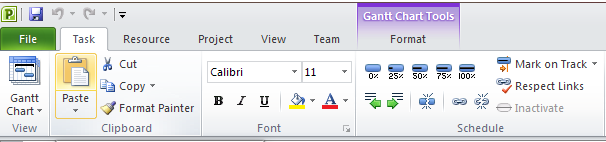
\includegraphics[scale=0.45]{Figuras/project_inicio1.png}
\caption{Guias de comandos e opções do \msp}
\label{fig:msp:tela1}
\end{figure}

\begin{figure}[!h]
\centering
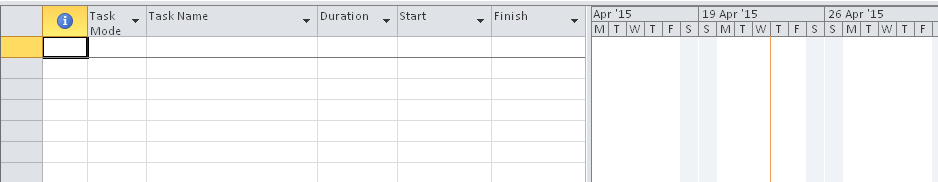
\includegraphics[scale=0.45]{Figuras/project_inicio2.png}
\caption{Tarefas e cronograma do \msp}
\label{fig:msp:tela2}
\end{figure}

Além do modo padrão de exibição, é possível escolher entre outros diversos modos e até mesmo criar o seu próprio modelo. Para isso, basta clicar no botão Gantt Chart (Figura \ref{fig:msp:tela3}) e selecionar um dos modos disponíveis.

\begin{figure}[!h]
\centering
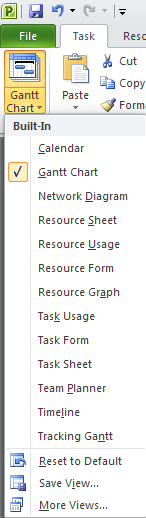
\includegraphics[scale=0.55]{Figuras/project_inicio3.png}
\caption{Botão para troca de modo de visualização}
\label{fig:msp:tela3}
\end{figure}
